
\section{Určenie náklonu zbrane}
Pre určenie náklonu zbrane v troch osách boli navrhnuté dve architektúry konvolučných neurónových sietí.
Každá z týchto sieti bola natrénovaná trikrát kvôli trom osám rotácie.
Nastavenia sieti boli opísane v návrhu.

Pre trénovanie v osi pitch bolo použitých 1036 obrázkov, na validáciu 222 a taktiež 222 pre testovanie presnosti siete.
V osi roll bolo na trénovanie použitých 3315 obrázkov, na validáciu 668 a 667 pre testovanie.
Nakoniec pre os yaw bolo použitých 3220 obrázkov na trénovanie a po 690 na validáciu a testovanie.
Všetky tieto obrázky prešli augmentáciou dát ako je opísane v \ref{subsec:augmentacia}.

\subsubsection{Pitch}
Sieť bola trénovaná v XX epochách.
Priebeh trénovania obydvoch sieti pre os Pitch je vidieť na obrázku \ref{pic:pitchaxis}.

\begin{figure}[H]
    \centering
    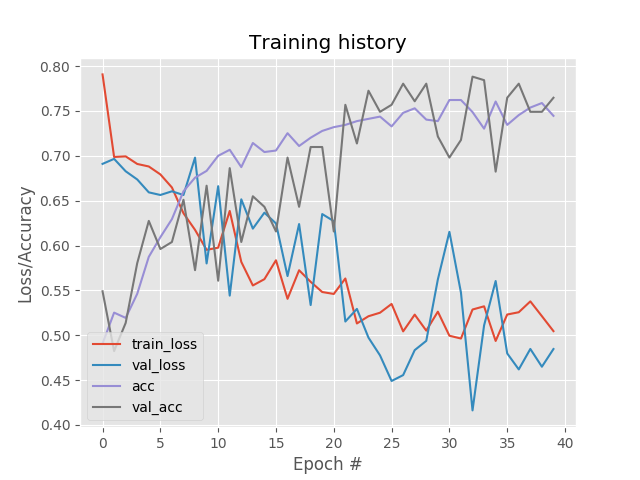
\includegraphics[width=0.75\textwidth]{alexnet-training_history} %alexnet-pitch-training_history
    \quad
	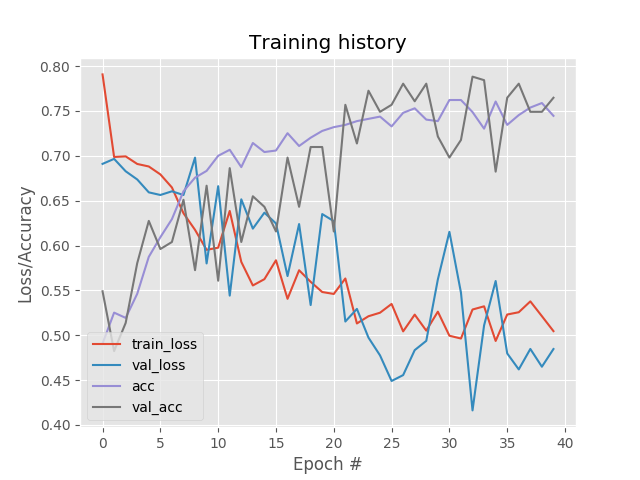
\includegraphics[width=0.75\textwidth]{alexnet-training_history} %vgglike-pitch-training_history
	\caption{Priebeh trénovania sieti AlexNetLike(vľavo) a VGGLike(vpravo).}
	\label{pic:pitchaxis}
\end{figure}

Výsledna presnosť sieti je uvedená v tabuľkách \ref{tab:alexnetpitchresults} a \ref{tab:vgglikepitchresults}.

\begin{table}[H]
    \centering
    \begin{tabular}{ccccc}
                                                                &                                    & \multicolumn{2}{c}{Klasifikované hodnoty}                                                         &                                    \\ \cline{3-5} 
                                                                & \multicolumn{1}{c|}{}              & \multicolumn{1}{c|}{Dlhé zbrane}                & \multicolumn{1}{c|}{Krátke zbrane}              & \multicolumn{1}{c|}{Úspešnosť}     \\ \cline{2-5} 
        \multicolumn{1}{c|}{}                                  & \multicolumn{1}{c|}{Dlhé zbrane}   & \multicolumn{1}{c|}{{\color[HTML]{009901} -}} & \multicolumn{1}{c|}{{\color[HTML]{9A0000} -}}  & \multicolumn{1}{c|}{\textbf{-\%}} \\ \cline{2-5} 
        \multicolumn{1}{c|}{\multirow{-2}{*}{Správne hodnoty}} & \multicolumn{1}{c|}{Krátke zbrane} & \multicolumn{1}{c|}{{\color[HTML]{9A0000} -}}  & \multicolumn{1}{c|}{{\color[HTML]{009901} -}} & \multicolumn{1}{c|}{\textbf{-\%}} \\ \cline{2-5} 
    \end{tabular}
    \caption{Výsledky natrénovanej siete AlexNetLike pre os Pitch.}
    \label{tab:alexnetpitchresults}
\end{table}

\begin{table}[H]
    \centering
    \begin{tabular}{ccccc}
                                                                &                                    & \multicolumn{2}{c}{Klasifikované hodnoty}                                                         &                                    \\ \cline{3-5} 
                                                                & \multicolumn{1}{c|}{}              & \multicolumn{1}{c|}{Dlhé zbrane}                & \multicolumn{1}{c|}{Krátke zbrane}              & \multicolumn{1}{c|}{Úspešnosť}     \\ \cline{2-5} 
        \multicolumn{1}{c|}{}                                  & \multicolumn{1}{c|}{Dlhé zbrane}   & \multicolumn{1}{c|}{{\color[HTML]{009901} -}} & \multicolumn{1}{c|}{{\color[HTML]{9A0000} -}}  & \multicolumn{1}{c|}{\textbf{-\%}} \\ \cline{2-5} 
        \multicolumn{1}{c|}{\multirow{-2}{*}{Správne hodnoty}} & \multicolumn{1}{c|}{Krátke zbrane} & \multicolumn{1}{c|}{{\color[HTML]{9A0000} -}}  & \multicolumn{1}{c|}{{\color[HTML]{009901} -}} & \multicolumn{1}{c|}{\textbf{-\%}} \\ \cline{2-5} 
    \end{tabular}
    \caption{Výsledky natrénovanej siete VGGLike pre os Pitch.}
    \label{tab:vgglikepitchresults}
\end{table}


\subsubsection{Roll}

\subsubsection{Yaw}
